% file: reasoning_case.tex
\begin{ReasoningBox}[title=Causal Discovery] % 可以通过 title 参数修改标题
    % --- 第一部分：问题描述与图片 ---
    % \begin{minipage}[t]{0.58\textwidth}
        \textbf{Question:} Based on the daily runoff water level time series data from 5 river sensors in East Germany, which adjacency matrix most accurately describes the causal relationship between them? In the matrix, columns represent 'cause' nodes, rows represent 'result' nodes, and '1' indicates the presence of causal effects.
    % \end{minipage}%
    % \hfill
    

    \vspace{0.5em}

    % --- 第二部分：选项 ---
    \textbf{Answer Choices:} 
    % \vspace{10pt}
    % --- Option A (Matrix 1: 3->2, 1->3, 4->3, 5->3) ---
    (A) \causalGraph{
    \draw[edge style] (2) -- (5);
    \draw[edge style] (2) -- (3);
    \draw[edge style] (3) -- (5);
    \draw[edge style] (4) -- (1);
} \hfill
% --- Option B (2->3, 2->4, 3->1, 4->5) ---
(B) \causalGraph{
    \draw[edge style] (2) -- (3);
    \draw[edge style] (2) -- (4);
    \draw[edge style] (3) -- (1);
    \draw[edge style] (4) -- (5);
} \hfill
% --- Option C (2->5, 3->1, 4->3, 4->4) ---
(C) \causalGraph{
    \draw[edge style] (2) -- (5);
    \draw[edge style] (3) -- (1);
    \draw[edge style] (4) -- (3);
    \draw[edge style] (4) -- (5);
} \hfill
% --- Option D (1->3, 3->2, 4->2, 5->4) ---
(D) \causalGraph{
    \draw[edge style] (1) -- (3);
    \draw[edge style] (3) -- (2);
    \draw[edge style] (4) -- (2);
    \draw[edge style] (5) -- (4);
}
    \vspace{10pt}
    \\
    \begin{wrapfigure}{r}{0.51\textwidth}
        \centering
        % wrapfigure 通常顶部会有多余空白，使用负 vspace 向上提，让图片和第一行文字对齐
        \vspace{-15pt} 
        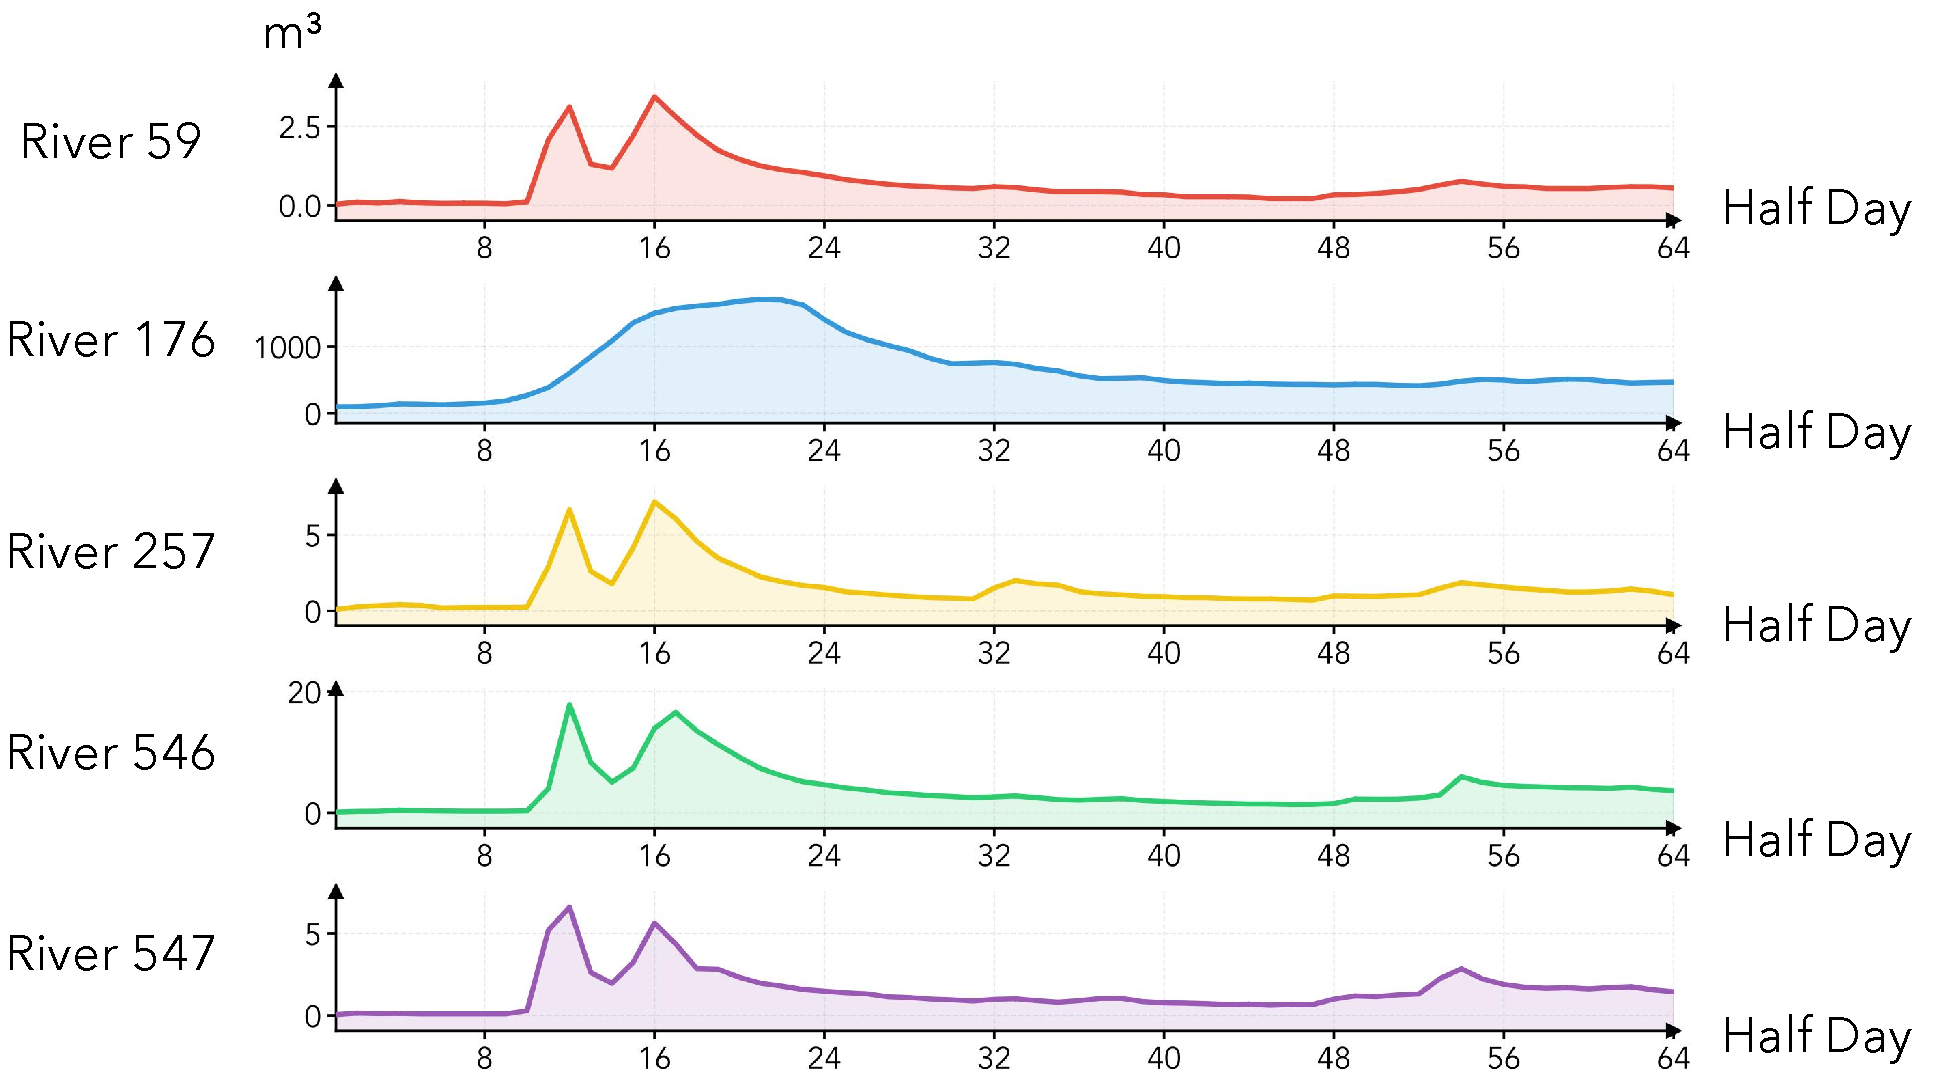
\includegraphics[width=\linewidth]{blocks/sample_cases_success/causal.pdf}
        % 调整底部的留白
        \vspace{-10pt}
    \end{wrapfigure}
    \textbf{Correct Answer:} \textcolor{correctgreen}{(B)} \\
    \\
    \vspace{10em}
    
    % --- 第四部分：基本原理 (Rationale) ---
   
\end{ReasoningBox}